% !TeX spellcheck = en_US
% !TeX encoding = UTF-8
% !TeX root = thesis.tex

\chapter{Reproducibility Record}
\label{app:reproducibility}

This appendix identifies the immutable inputs, configurations, checkpoints, and evidence used by the method in Chapter~\ref{chap:methods}. It is a reproduction record for the executed repository state, not a claim that a fresh clone contains the licensed dataset or all large artifacts. Paths are relative to the repository root unless stated otherwise. SHA-256 is used for direct files; feature-store identities hash the ordered list of shard paths and their individual SHA-256 values.

\section{Software and Hardware Scope}
\label{app:environment}

The official Stage-2 run manifests record the environment shown in the first column of Table~\ref{tab:environment}. Versions absent from those manifests are not retroactively assigned to training. The second column is the host observed during an environment audit on 5 September 2026 and again for later compatibility work on 19 September 2026. The later observation documents the environment used to replay and extend the frozen representation; it is not evidence that every earlier stage used every listed package version.

\begin{table}[tbp]
    \centering
    \small
    \caption[Recorded and observed environments.]{Recorded training environment versus the later observed host. Shared system RAM is not counted as CUDA VRAM.}
    \label{tab:environment}
    \begin{tabularx}{\textwidth}{@{}l>{\raggedright\arraybackslash}X>{\raggedright\arraybackslash}X@{}}
        \toprule
        \textbf{Item} & \textbf{Official Stage-2 manifests} & \textbf{Later observed host} \\
        \midrule
        Operating context & Linux 5.15.167.4, WSL2, x86-64, glibc 2.39 & Ubuntu 24.04.3 LTS under WSL2; same kernel family and architecture \\
        Python & 3.12.3 & 3.12.3 \\
        PyTorch & 2.5.1+cu121 & 2.5.1+cu121 \\
        CUDA / cuDNN & Torch build suffix records CUDA 12.1; cuDNN not recorded & Torch runtime 12.1; cuDNN 9.1.0 \\
        NumPy / PyYAML & 1.26.4 / 6.0.2 & 1.26.4 / 6.0.2 \\
        Additional packages & Not recorded & Torchvision 0.20.1+cu121; OpenCV 4.10.0.84; Transformers 5.12.0; PEFT 0.19.1; scikit-learn 1.8.0; SciPy 1.17.0 \\
        GPU & NVIDIA GeForce RTX 4050 Laptop GPU & Same; 6,141 MiB dedicated memory by \code{nvidia-smi} \\
        Driver & Not recorded & 591.66 \\
        Source state & Commit \hashvalue{75ef4dfc1c839b1b1a10}{0cc291904be5c9e1dec4}; dirty tree & Later phase-specific repository states; evidence paths and hashes control the named outputs \\
        \bottomrule
    \end{tabularx}
\end{table}

The development repository's \code{requirements.txt} at commit \code{072dac2} has SHA-256 \hashvalue{d6668f61b80a38595384edb3e5673be3}{e7f7ac1b6f385a44fbc8465397a29da9}. It pins PyTorch 2.3.1 and Torchvision 0.18.1. By contrast, the manifests and live host record PyTorch 2.5.1+cu121, while the live host records Torchvision 0.20.1+cu121. Several other libraries are lower-bounded or unpinned. The mismatch is disclosed rather than rewriting the requirements file and falsely presenting a later environment as the historical training lock.

The Stage-1b adapter checkpoint, log, and source configuration reconstruct the implemented training method, but no contemporaneous resolved run manifest captured its complete software environment. The extraction benchmark measured bounded offline clip extraction on the local GPU. It is not a measurement of live-stream latency, multi-stream capacity, or deployment throughput.

\section{Artifact Identities and Relationships}
\label{app:artifact-identities}

The dataset partition and clip index, the LoRA checkpoint and its source configuration, the sparse and dense feature-store identities, the normal-prototype and prototype-distance tensors, and the three per-seed Stage-2 resolved configurations and selected checkpoints are each fixed and identified by a SHA-256 hash. These hashes, and the file and directory paths they identify, are recorded in \path{reproducibility/PROVENANCE.md} rather than reproduced here. The active response model consumes the LoRA-derived prototype artifact, not the separate historical frozen-backbone prototype store. The teacher directory named there was subsequently overwritten in place with LoRA-derived scores; the frozen originals are preserved alongside it as \code{*.frozen\_backup} files, so the description of teacher-score construction in Chapter~\ref{chap:methods} is historically correct for the executed run but is not reproducible from the current configuration files alone.

The dense test feature manifest is \path{data/ucf_crime/artifacts/dman_v21/features_lora_temporal_system_v1/manifest.json}, SHA-256 \hashvalue{4385c610f53c8c1df041499e97d88202}{fc83ffbc7337ef08b3a0e5171477cb36}. It lists 135 shards and 69,090 clips; the store identity is \hashvalue{a2d1667f96c72a6918b87d932838fca0}{0caca3b611f37e2fcdc7a664ea77ee7c}. Its prototype-distance tensor is \path{artifacts/stage2/teacher_temporal_system_v1/teacher_scores_test.pt}, SHA-256 \hashvalue{398c53c42fdc242f012d475ac4c3433e6}{780c03b024ba90e933ca40ae99d32e5}.

The canonical evidence chain is:

\begin{itemize}
    \item fixed-bag summary: \path{reproducibility/evidence/dispatch_repro_v1/summary.json}, SHA-256 \hashvalue{ffb1e5d12ba1922a0e21e01eacab83ec}{d031a9ecc309e26df8a2ea0bea512b5c};
    \item validation-only prototype-distance study: \path{artifacts/stage2/evidence/teacher_ablation_v1/summary.json}, SHA-256 \hashvalue{edd6bda5065a1dea085a884f46ea5d81}{e79c0109796d9a266c1ee62819b89798};
    \item validation-only normal-bag response-loss study: \path{reproducibility/evidence/normal_bag_response_study/summary.json}, SHA-256 \hashvalue{8123b0bec4e1da314b013fcb4e423e87}{1b625231994501f2fd4ca3f71e9b6865}, with its per-run configuration, checkpoint, and evaluation hashes in \path{reproducibility/PROVENANCE.md};
    \item dense temporal/system evaluation: \path{artifacts/stage2/evidence/temporal_system_v1/summary.json}, SHA-256 \hashvalue{41f219f41474bdce58d0479e1d39e72a}{02811819564fbf4cee4d05d5031575d8};
    \item final quantitative authority: \path{artifacts/stage2/evidence/canonical_thesis_v1/package.json}, SHA-256 \hashvalue{346ad82324c95db37fbbc92685c57ff31}{6436f5237db29368196461e253a1a78}.
\end{itemize}

The 16 canonical vector figures under \path{artifacts/thesis_figures/phase6/} were generated from the final package by \path{utils/generate_phase6_figures.py}, SHA-256 \hashvalue{24264eedfb2cd2a6776c752d7fb07e9f}{d5c58f4f1f8429b60168e2f58e10234c}; Figure~\ref{fig:results-cad-example} was later regenerated from the same package with layout changes only, by the script version with SHA-256 \hashvalue{7a3834bf90812ae04bd5e2e074cfe6f0}{fe8a0d74b93d7f29d85ab75ed7eeef0b}. Figures~\ref{fig:results-joint-dispatch}, \ref{fig:results-routing-comparison}, \ref{fig:results-qualitative}, and \ref{fig:results-temporal-category} were drawn for the final revision by \path{utils/generate_revision_figures.py} from the same package and the dense per-video records it lists, whose hashes the script checks. Figures~\ref{fig:method-overview} and~\ref{fig:protocol-overview} are drawn directly in the thesis source and contain no measured values. The bootstrap intervals in Chapter~\ref{chap:results} were computed by \path{utils/bootstrap_test_cis.py} from the same package and records and are stored in \path{artifacts/stage2/evidence/bootstrap_v1/bootstrap_cis.json}. The hashes of all figure files included in the thesis are recorded in \path{reproducibility/PROVENANCE.md}.

\section{Command Record}
\label{app:commands}

The exact entry-point commands for adaptation training, sparse and dense feature extraction, Stage-2 training and evaluation for each of the three official seeds, evidence verification, canonical-package and figure generation, and the controlled document build are recorded in \path{reproducibility/PROVENANCE.md}, together with the source-defined command form for each stage and the protected output locations that must not be overwritten by re-execution.

\section{Determinism and Remaining Limitations}
\label{app:repro-limits}

Fixed split files, fixed validation and test bag manifests, resolved run configurations, selected checkpoints, thresholds, and the temporal protocol are immutable inputs. Stage-2 training seeds are 1337, 2027, and 3407; evaluation seed 1337 is shared. Temporal random-reference scores use one SHA-256-derived PCG64 draw per video and are reused across checkpoints. The final summaries require all 290 routing videos, all 870 checkpoint--video records, all 69,090 dense clips, and zero unresolved technical failures.

The following boundaries remain material:

\begin{itemize}
    \item raw data, checkpoints, feature shards, prototype-distance tensors, and dense evidence are local and largely Git-ignored; no external archive URI or upload receipt exists; a fresh clone with the local evidence bundle passes the evidence verifiers, but raw videos and feature stores are not part of that check;
    \item the raw dataset was not hashed as one distributable object, and lawful access to UCF-Crime remains a prerequisite;
    \item the official Stage-2 runs were executed at commit \code{75ef4df} with uncommitted changes in the working tree, and the Stage-2 trainer was extended afterwards; checking out that commit does not reproduce the executed code, so the named inputs and outputs are identified by their recorded artifact hashes and store identities rather than by the commit;
    \item the Stage-1b environment is incomplete and the standard sparse subset cannot be regenerated from configuration alone because the startup Python hash seed was not captured;
    \item the retained Transformers 5.12.0 loader ignores legacy cached VideoMAE \code{q\_bias} and \code{v\_bias} keys and leaves 36 newly represented linear biases at zero; retaining it reproduces 18 stored validation embeddings with maximum absolute difference $9.765625\times10^{-4}$ and minimum cosine similarity $0.9999997616$, while restoring the published bias tensors does not, so it is a verified compatibility choice, not a reconstruction of all published VideoMAE bias tensors;
    \item persisted \code{float16} prototypes approximate unavailable original \code{float32} centers;
    \item five source-boundary conflicts remain uncorrected and are excluded only from temporal metrics;
    \item three Stage-2 seeds support descriptive mean and sample standard deviation, not inferential significance; and
    \item the test outcomes were previously inspected, while CAD output remains an offline demonstration with no live, external, reliability, or safety validation.
\end{itemize}

These limitations do not prevent verification of the named local evidence. They do limit claims of complete portability, untouched-test evaluation, historical environment reconstruction, and operational reproducibility.

\section{Temporal Average Precision by Category}
\label{app:temporal-category}

\begin{figure}[htbp]
    \centering
    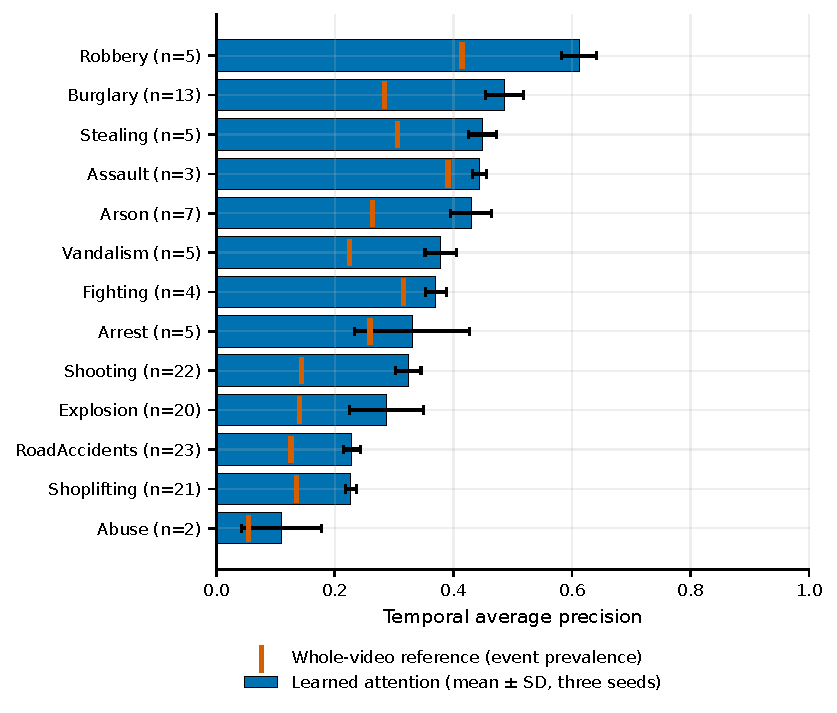
\includegraphics[width=0.9\textwidth]{fig_temporal_ap_by_category_r20.pdf}
    \caption[Temporal AP by anomaly category.]{Dense indexed temporal AP by anomaly category for the 135 source-bounded anomalous test videos (mean and sample SD over three seeds; $n$ is the number of videos). The orange mark is the whole-video reference, which equals the category's mean event prevalence. Most categories contain fewer than ten videos, so the ordering is not a ranking.}
    \label{fig:results-temporal-category}
\end{figure}

